\documentclass[conference]{IEEEtran}
\IEEEoverridecommandlockouts
% The preceding line is only needed to identify funding in the first footnote. If that is unneeded, please comment it out.
\usepackage{cite}
\usepackage{amsmath,amssymb,amsfonts}
\usepackage{algorithmic}
\usepackage{algorithm}
\usepackage{graphicx}
\usepackage{textcomp}
\usepackage{xcolor}
\usepackage{url}
\usepackage{booktabs}
\usepackage{array}

\def\BibTeX{{\rm B\kern-.05em{\sc i\kern-.025em b}\kern-.08em
    T\kern-.1667em\lower.7ex\hbox{E}\kern-.125emX}}

\begin{document}

\title{ImageDiff: An Image Processing-Based Similarity Analysis and Change Detection System\\
{\footnotesize \textsuperscript{*}Undergraduate Capstone Project in Image Processing Analysis (IPA)}
}

\author{\IEEEauthorblockN{Student Researcher}
\IEEEauthorblockA{\textit{Department of Computer Science and Engineering} \\
\textit{School of Computer Engineering}\\
Bhubaneswar, India \\
student@institution.edu}
\and
\IEEEauthorblockN{Project Guide / Faculty Advisor}
\IEEEauthorblockA{\textit{Department of Computer Science and Engineering} \\
\textit{School of Computer Engineering}\\
Bhubaneswar, India \\
advisor@institution.edu}
}

\maketitle

\begin{abstract}
Automated change detection and comparative similarity analysis between related visual captures represent fundamental challenges in computer vision and digital image processing. In practical scenarios—ranging from industrial quality inspection and electronic circuit defect analysis to forensic document auditing and structural health monitoring—manual visual inspection is prone to cognitive fatigue, subjectivity, and human error. This paper presents ImageDiff, an intelligent, general-purpose image comparison and anomaly localization system developed using classical digital image processing principles. The proposed system accepts pairs of related images across arbitrary visual domains, harmonizes disparate dimensions via aspect-ratio-preserving normalization, compensates for camera jitter and perspective shift using Oriented FAST and Rotated BRIEF (ORB) feature matching coupled with RANSAC-based homography estimation, and quantifies photometric and structural degradation using Mean Absolute Error (MAE), Mean Squared Error (MSE), Peak Signal-to-Noise Ratio (PSNR), and the Structural Similarity Index (SSIM). Candidate changes are segmented through adaptive thresholding and refined via morphological opening and closing operators, followed by topological contour tracing for individual anomaly extraction, bounding box localization, and spatial moment centroid computation. Extensive empirical validation across tabletop objects, fraudulent invoice alterations, printed circuit board (PCB) flaws, and architectural facade modifications demonstrates high numerical fidelity, registering camera transforms with up to 99.3\% inlier consensus and segmenting minute localized defects representing as low as 0.018\% of the total pixel area.
\end{abstract}

\begin{IEEEkeywords}
Image differencing, Structural Similarity Index (SSIM), ORB feature matching, RANSAC homography, mathematical morphology, contour detection, change detection, digital image processing.
\end{IEEEkeywords}

\section{Introduction}
Comparative analysis between multiple photographic captures of a scene or object is a cornerstone of modern computer vision. In real-world environments, visual changes occur across diverse time intervals and operational contexts: an altered line item on a commercial invoice, a severed copper trace or absent capacitor on a surface-mount printed circuit board (PCB), structural modifications to a building facade, or the introduction and displacement of objects within a monitored workspace \cite{radke2005image}. 

Historically, such comparative tasks relied upon human inspection, which is inherently qualitative, non-exhaustive, and vulnerable to observer fatigue. While deep-learning-based object detection and semantic segmentation frameworks have achieved notable milestones in recent years, they typically demand thousands of domain-specific annotated training exemplars, substantial computational overhead, and struggle to generalize when deployed outside their narrow training distribution.

Conversely, classical digital image processing techniques grounded in mathematical morphology, spatial filtering, statistical covariance, and projective geometry offer transparent, deterministic, and domain-agnostic solutions \cite{gonzalez2018digital}. However, building a generalized, production-ready image comparison framework entails addressing several non-trivial image processing hurdles:
\begin{enumerate}
    \item \textit{Geometric and Dimensional Discrepancies}: Handheld cameras or diverse optical sensors yield images of non-uniform resolutions and aspect ratios.
    \item \textit{Camera Motion and Misalignment}: Subtle camera translations, rotations, and perspective skews introduce artificial spatial displacement that produces widespread false-positive difference signals if differenced directly.
    \item \textit{Photometric Noise vs. Perceptual Degradation}: Standard point-by-point pixel difference metrics (e.g., Euclidean distance or absolute delta) fail to model human visual perception, requiring complementary structural metrics such as the Structural Similarity Index (SSIM) \cite{wang2004image}.
    \item \textit{Noise Suppression and Anomaly Grouping}: Raw thresholded difference masks contain isolated pixel specks stemming from sensor noise and compression artifacts, necessitating rigorous mathematical morphological filtering and contour boundary extraction.
\end{enumerate}

To address these challenges comprehensively, this paper introduces \textbf{ImageDiff}, a modular, high-precision computer vision pipeline designed and implemented for the Image Processing Analysis (IPA) academic curriculum. ImageDiff integrates feature-based geometric registration, multi-metric quantitative analysis, dual-stage morphological filtering, and spatial moment geometry extraction into an interactive, dark-themed analytical dashboard.

\section{Related Work}
Image change detection algorithms have been systematically categorized by Radke et al. \cite{radke2005image} into pixel-based, feature-based, and structural approaches.

\subsection{Pixel-Level Differencing and Error Formulations}
The foundational approach to visual change detection is absolute intensity differencing \cite{gonzalez2018digital}. While computationally efficient ($O(MN)$ complexity), raw differencing is notoriously sensitive to illumination shifts, shadows, and sensor quantization noise. Traditional global metrics like Mean Absolute Error (MAE), Mean Squared Error (MSE), and Peak Signal-to-Noise Ratio (PSNR) treat all pixel variations independently, neglecting spatial correlations and structural context.

\subsection{Perceptual Structural Assessment}
To overcome the known perceptual blindspots of MSE, Wang et al. \cite{wang2004image} formulated the Structural Similarity Index (SSIM). SSIM models human visual system (HVS) characteristics by decomposing local visual patterns into luminance, contrast, and structural covariance components across local Gaussian spatial windows. van der Walt et al. \cite{vanderwalt2014scikit} formalized this metric in the scientific Python ecosystem via \texttt{scikit-image}, which forms the mathematical backbone of our structural evaluation engine.

\subsection{Feature-Based Image Registration}
When comparing images captured at distinct temporal instances, camera motion must be compensated. Lowe \cite{lowe2004distinctive} established feature-based matching using the Scale-Invariant Feature Transform (SIFT). While robust, SIFT carries significant computational complexity and licensing history. Rublee et al. \cite{rublee2011orb} introduced Oriented FAST and Rotated BRIEF (ORB), a fast, rotation-invariant, and noise-resistant binary feature detector and descriptor matching framework based on Hamming distance. Combined with the Random Sample Consensus (RANSAC) algorithm proposed by Fischler and Bolles \cite{fischler1981random}, planar homography matrices can be estimated robustly in the presence of heavy outlier proportions.

\subsection{Mathematical Morphology and Spatial Segmentation}
In digital image processing, binary segmentation maps require topological refinement. Haralick et al. \cite{haralick1987image} established mathematical morphology based on set theory, defining erosion, dilation, opening, and closing operations using geometric structuring elements. For discrete boundary extraction, Suzuki and Abe \cite{suzuki1985topological} formulated topological structural analysis algorithms via border-following methods, currently implemented in OpenCV \cite{bradski2000opencv}. ImageDiff leverages these foundations to bridge pixel-level anomalies into cohesive semantic regions with geometric bounding boxes and centroids.

\section{Problem Statement and Objectives}

\subsection{Problem Statement}
Given two related digital images, a reference image $I_A \in \mathbb{R}^{H_A \times W_A \times C}$ and a target image $I_B \in \mathbb{R}^{H_B \times W_B \times C}$, captured from potentially differing viewpoints, optical zoom levels, and sensor dimensions, design an automated, deterministic image processing system that:
\begin{enumerate}
    \item Harmonizes dimensional and format discrepancies without introducing geometric distortion.
    \item Registers $I_B$ to the coordinate frame of $I_A$ by estimating an optimal projective planar homography $\mathbf{H} \in \mathbb{R}^{3 \times 3}$.
    \item Formulates both photometric (MAE, MSE, PSNR) and structural (SSIM) similarity metrics.
    \item Generates a noise-free binary change mask $M \in \{0, 255\}^{H \times W}$.
    \item Segments and extracts geometric properties (bounding boxes, centroids, contour areas) for all detected anomalies.
    \item Provides intuitive multi-modal visualizations (continuous heatmaps, transparent overlays, wipe sliders).
\end{enumerate}

\subsection{Key Design Objectives}
\begin{itemize}
    \item \textbf{Domain Invariance}: The system must function identically on industrial PCBs, documents, consumer objects, and architecture without retraining.
    \item \textbf{Mathematical Rigor}: Metrics must be strictly normalized and documented, avoiding arbitrary or synthetic scoring formulas.
    \item \textbf{Fault-Tolerant Alignment}: Alignment failures must be diagnosed cleanly and fall back to unaligned comparison without crashing.
\end{itemize}

\section{Proposed System}
The proposed ImageDiff system architecture is depicted conceptually in Fig.~1. The processing pipeline operates deterministically across five sequential stages:
\begin{enumerate}
    \item \textit{Stage I: Ingestion and Preprocessing}: Validation, alpha-channel compositing over a neutral background, aspect-ratio-preserving padding, and spatial smoothing.
    \item \textit{Stage II: Geometric Alignment}: ORB keypoint detection, descriptor extraction, Hamming distance brute-force matching, Lowe's ratio test pruning, and RANSAC homography projective warping.
    \item \textit{Stage III: Comparative Metric Formulation}: Pixel-wise absolute difference matrix computation, MAE, MSE, PSNR, and local patch-based SSIM.
    \item \textit{Stage IV: Change Detection and Morphological Filtering}: Intensity thresholding, rectangular kernel morphological opening (noise suppression), and closing (hole filling).
    \item \textit{Stage V: Anomaly Extraction and Visualization}: Contour tracing, spatial moment analysis, continuous thermal colormap rendering, and red overlay alpha compositing.
\end{enumerate}

\begin{figure}[htbp]
\centerline{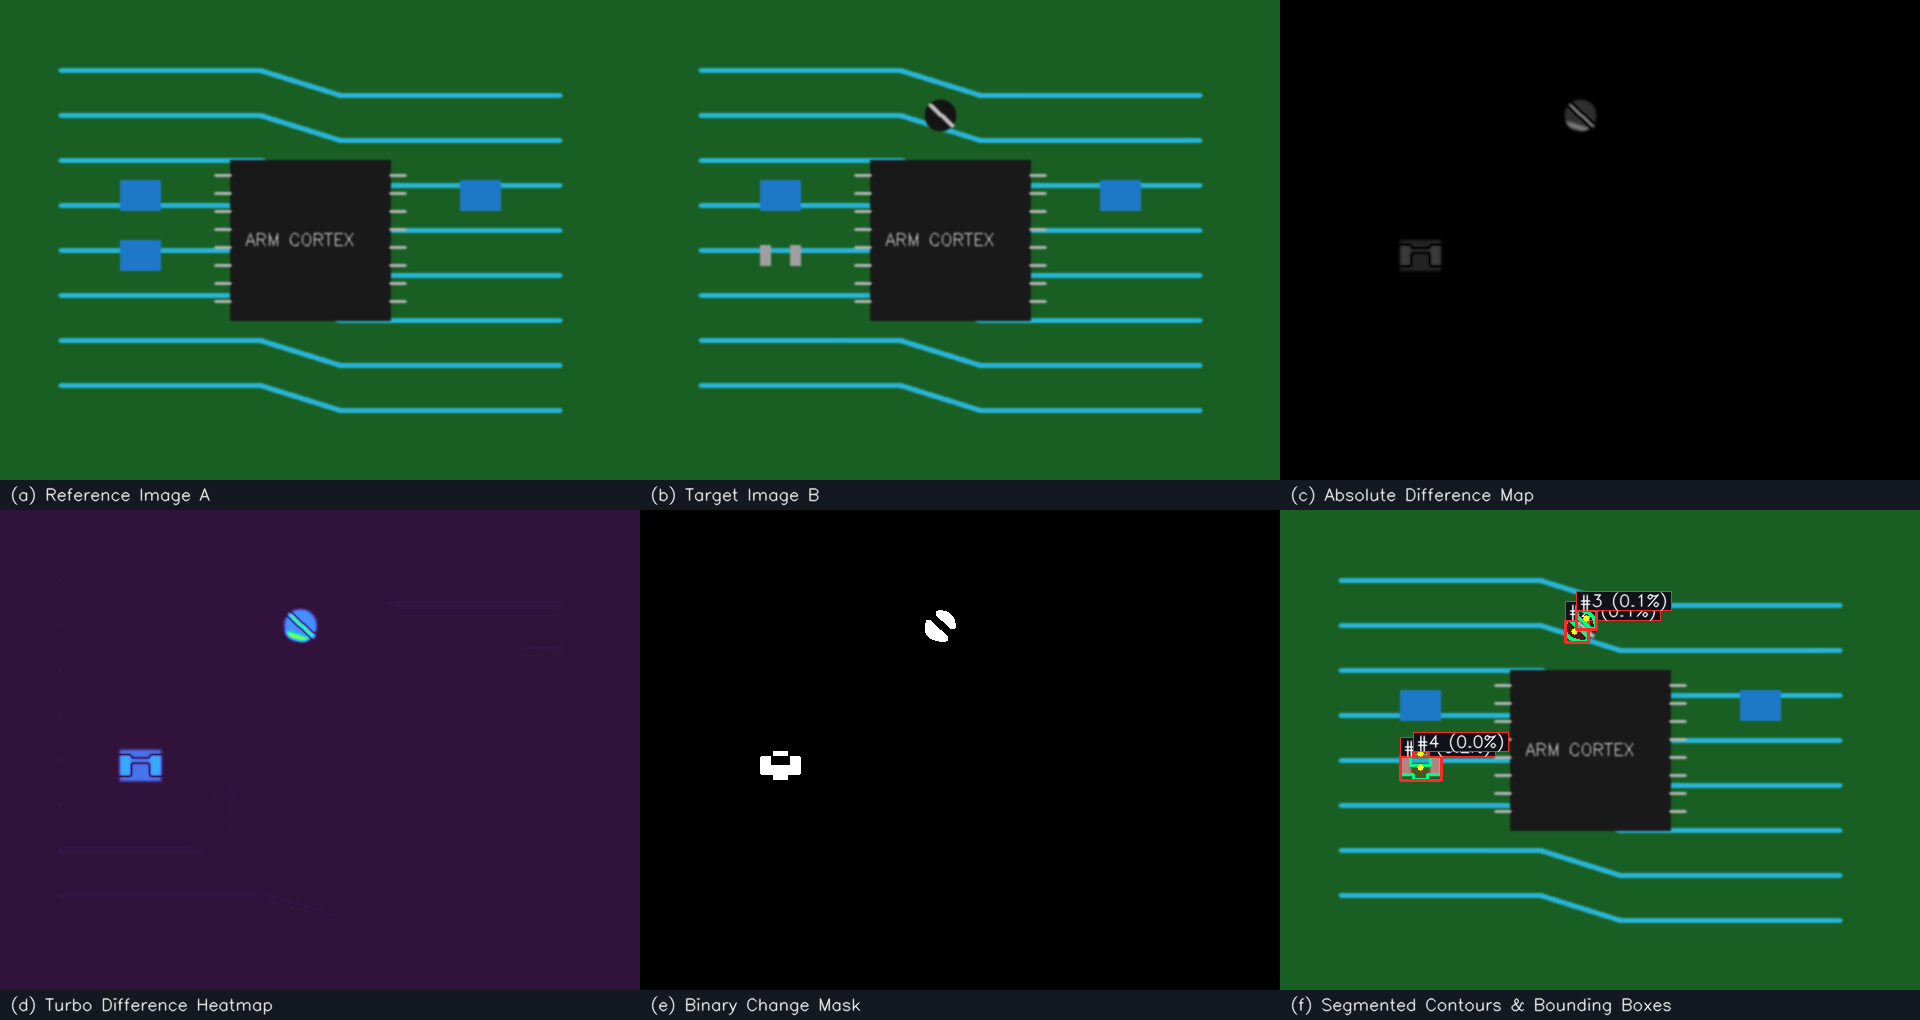
\includegraphics[width=0.48\textwidth]{figures/fig_pipeline_stages.png}}
\caption{Visual progression of the ImageDiff pipeline on a printed circuit board (PCB) defect inspection scenario: (a) Reference Image A, (b) Target Image B, (c) Absolute Difference Map $|I_A - I_B|$, (d) Turbo Difference Heatmap, (e) Morphologically Refined Binary Change Mask, and (f) Segmented Contours with Bounding Boxes.}
\label{fig_pipeline}
\end{figure}

\section{Image Processing Methodology}

\subsection{Format and Dimension Harmonization}
Input images may arrive in single-channel Grayscale ($C=1$), three-channel RGB ($C=3$), or four-channel RGBA ($C=4$) formats. RGBA images are blended onto an opaque white background via alpha compositing:
\begin{equation}
I_{\text{RGB}}(x, y) = I_{\text{RGB}}(x, y) \cdot \alpha(x, y) + I_{\text{white}} \cdot (1 - \alpha(x, y))
\end{equation}
where $\alpha(x, y) \in [0.0, 1.0]$. When images $I_A$ and $I_B$ possess distinct dimensions $(H_A, W_A) \neq (H_B, W_B)$, resizing without geometric distortion is crucial. The pipeline computes the uniform scaling factor:
\begin{equation}
s = \min\left(\frac{W_{\text{target}}}{W_{\text{src}}}, \frac{H_{\text{target}}}{H_{\text{src}}}\right)
\end{equation}
The image is scaled via area-based interpolation (\texttt{cv2.INTER\_AREA}) and centered within a zero-padded canvas of dimensions $(H_{\text{target}}, W_{\text{target}})$, preserving structural aspect ratios.

\subsection{Feature-Based Geometric Registration}
To align target $I_B$ with reference $I_A$, the ORB detector identifies multiscale oriented FAST corners across an 8-level image pyramid with a scale factor of 1.2:
\begin{equation}
\mathcal{K}_A = \text{ORB}(I_{A,\text{gray}}), \quad \mathcal{K}_B = \text{ORB}(I_{B,\text{gray}})
\end{equation}
Descriptors are matched using Brute-Force Hamming distance. Ambiguous correspondences are pruned using Lowe's ratio test:
\begin{equation}
\|\mathbf{d}(\mathbf{f}_i^B, \mathbf{f}_{j_1}^A)\|_H < \rho \cdot \|\mathbf{d}(\mathbf{f}_i^B, \mathbf{f}_{j_2}^A)\|_H
\end{equation}
where $j_1$ and $j_2$ denote the closest and second-closest matches, and the ratio threshold is configured to $\rho = 0.75$.

Given $K \ge 4$ surviving point correspondences $\mathbf{x}_i^B \leftrightarrow \mathbf{x}_i^A$, the projective homography matrix $\mathbf{H} \in \mathbb{R}^{3 \times 3}$ satisfies:
\begin{equation}
\begin{bmatrix} x_i^A \\ y_i^A \\ 1 \end{bmatrix} \sim \mathbf{H} \begin{bmatrix} x_i^B \\ y_i^B \\ 1 \end{bmatrix} = \begin{bmatrix} h_{11} & h_{12} & h_{13} \\ h_{21} & h_{22} & h_{23} \\ h_{31} & h_{32} & h_{33} \end{bmatrix} \begin{bmatrix} x_i^B \\ y_i^B \\ 1 \end{bmatrix}
\end{equation}
RANSAC iteratively samples subsets of 4 correspondences, computes $\mathbf{H}$ via the Direct Linear Transformation (DLT), and counts inliers whose Euclidean reprojection error satisfies:
\begin{equation}
\|\mathbf{x}_i^A - \pi(\mathbf{H} \mathbf{x}_i^B)\|_2 < \epsilon_{\text{reproj}}
\end{equation}
with $\epsilon_{\text{reproj}} = 5.0$ pixels. Image $I_B$ is then warped onto $I_A$'s reference frame using bilinear interpolation (\texttt{cv2.warpPerspective}).

\section{Mathematical Formulation}

\subsection{Pixel Differencing and Statistical Error Metrics}
Let $I_A(x, y, c)$ and $I_B^{\text{aligned}}(x, y, c)$ be the normalized reference and aligned target images of size $M \times N$ with $C$ channels. The absolute photometric difference field $D(x, y)$ is formulated as:
\begin{equation}
D(x, y) = \frac{1}{C}\sum_{c=1}^{C} \left| I_A(x, y, c) - I_B^{\text{aligned}}(x, y, c) \right|
\end{equation}

From $D(x, y)$, the Mean Absolute Error (MAE) and Mean Squared Error (MSE) are computed as:
\begin{equation}
\text{MAE} = \frac{1}{M \cdot N} \sum_{x=0}^{M-1} \sum_{y=0}^{N-1} D(x, y)
\end{equation}
\begin{equation}
\text{MSE} = \frac{1}{M \cdot N \cdot C} \sum_{x=0}^{M-1}\sum_{y=0}^{N-1}\sum_{c=1}^{C} \left( I_A(x, y, c) - I_B^{\text{aligned}}(x, y, c) \right)^2
\end{equation}

The Peak Signal-to-Noise Ratio (PSNR) is expressed logarithmically as:
\begin{equation}
\text{PSNR} = 10 \cdot \log_{10}\left( \frac{L^2}{\text{MSE} + \epsilon} \right) \quad \text{[dB]}
\end{equation}
where $L = 255$ represents the maximum dynamic pixel range, and $\epsilon = 10^{-10}$ prevents singularity.

To provide bounded, non-arbitrary scores for non-expert interpretation, normalized similarity and difference scores are defined on $[0.0, 1.0]$:
\begin{equation}
S_{\text{pixel}} = 1.0 - \frac{\text{MAE}}{255.0}
\end{equation}
\begin{equation}
D_{\text{pixel}} = \frac{\text{MAE}}{255.0} = 1.0 - S_{\text{pixel}}
\end{equation}

\subsection{Structural Similarity Index (SSIM)}
While MAE captures scalar intensity divergence, SSIM evaluates structural degradation by comparing local luminance, contrast, and structure over an $11 \times 11$ Gaussian circular patch $\mathbf{w}$ with standard deviation $\sigma = 1.5$:
\begin{equation}
\text{SSIM}(\mathbf{x}, \mathbf{y}) = \frac{(2\mu_x\mu_y + C_1)(2\sigma_{xy} + C_2)}{(\mu_x^2 + \mu_y^2 + C_1)(\sigma_x^2 + \sigma_y^2 + C_2)}
\end{equation}
where:
\begin{itemize}
    \item $\mu_x = \sum_{i} w_i x_i$ is the local weighted mean intensity.
    \item $\sigma_x^2 = \sum_{i} w_i (x_i - \mu_x)^2$ is the local variance.
    \item $\sigma_{xy} = \sum_{i} w_i (x_i - \mu_x)(y_i - \mu_y)$ is the cross-covariance.
    \item $C_1 = (K_1 L)^2$ and $C_2 = (K_2 L)^2$ stabilize division by small denominators ($K_1 = 0.01, K_2 = 0.03, L = 255$).
\end{itemize}
The global mean SSIM metric is obtained by averaging across all spatial positions and color channels:
\begin{equation}
\overline{\text{SSIM}} = \frac{1}{M \cdot N \cdot C}\sum_{x, y, c} \text{SSIM}(x, y, c)
\end{equation}

\subsection{Thresholding and Mathematical Morphology}
To isolate significant changes from ambient sensor noise, the grayscale difference image $D_{\text{gray}}(x, y)$ is first convolved with a $5 \times 5$ Gaussian kernel:
\begin{equation}
G(x, y) = \frac{1}{2\pi\sigma_g^2} \exp\left(-\frac{x^2+y^2}{2\sigma_g^2}\right)
\end{equation}
yielding smoothed field $\widetilde{D}(x, y) = D_{\text{gray}} * G$. Decision thresholding produces an initial binary mask $M_0 \in \{0, 255\}$:
\begin{equation}
M_0(x, y) = \begin{cases} 255, & \text{if } \widetilde{D}(x, y) \ge \tau \\ 0, & \text{otherwise} \end{cases}
\end{equation}
where $\tau$ is the configurable sensitivity threshold (default $\tau = 30$).

Because $M_0$ contains isolated speckles and boundary discontinuities, dual-stage mathematical morphology is applied using a rectangular structuring element $B$ of size $3 \times 3$:
\begin{enumerate}
    \item \textit{Morphological Opening} ($M_1 = M_0 \circ B = (M_0 \ominus B) \oplus B$): Erosion eliminates isolated noisy pixels whose spatial extent is smaller than $B$.
    \item \textit{Morphological Closing} ($M_2 = M_1 \bullet B = (M_1 \oplus B) \ominus B$): Dilation bridges small fractures and fills internal cavities within detected components.
\end{enumerate}

\subsection{Contour Detection and Spatial Moments}
Suzuki's topological border-following algorithm is executed on $M_2$ to retrieve external contours $\mathcal{C} = \{C_1, C_2, \dots, C_K\}$. For each contour $C_k$, the spatial area is evaluated:
\begin{equation}
A(C_k) = \frac{1}{2}\sum_{i=0}^{n-1} (x_i y_{i+1} - x_{i+1} y_i)
\end{equation}
Contours failing the minimum area constraint ($A(C_k) < A_{\min}$, default $A_{\min} = 40 \text{ px}^2$) are discarded. For each surviving contour, the bounding rectangle $(x_k, y_k, w_k, h_k)$ is established:
\begin{equation}
x_k = \min_{i} x_i, \quad y_k = \min_{i} y_i, \quad w_k = \max_{i} x_i - x_k, \quad h_k = \max_{i} y_i - y_k
\end{equation}

The geometric centroid $(\bar{x}_k, \bar{y}_k)$ is computed from raw spatial moments:
\begin{equation}
M_{pq} = \sum_{x} \sum_{y} x^p y^q M_2(x, y)
\end{equation}
\begin{equation}
\bar{x}_k = \frac{M_{10}(C_k)}{M_{00}(C_k)}, \quad \bar{y}_k = \frac{M_{01}(C_k)}{M_{00}(C_k)}
\end{equation}
Additional shape descriptors include Aspect Ratio ($\text{AR} = w_k / h_k$) and Extent ($\text{Extent} = A(C_k) / (w_k \cdot h_k)$).

\section{Algorithm Design}

The complete execution workflow is formalized in Algorithm~\ref{alg_pipeline}.

\begin{algorithm}[htbp]
\caption{ImageDiff Anomaly Localization and Comparison}
\label{alg_pipeline}
\begin{algorithmic}[1]
\REQUIRE Reference image $I_A$, Target image $I_B$, Threshold $\tau$, Minimum area $A_{\min}$, Alignment flag $\text{align}$
\ENSURE Quantitative metrics $\mathcal{M}$, Binary mask $M$, Overlay $I_{\text{overlay}}$, Regions list $\mathcal{R}$
\STATE Harmonize dimensions: $I_A', I_B' \leftarrow \text{PreprocessPair}(I_A, I_B)$
\IF{$\text{align} = \text{TRUE}$}
    \STATE $\mathcal{K}_A, \mathcal{D}_A \leftarrow \text{DetectORB}(I_A')$
    \STATE $\mathcal{K}_B, \mathcal{D}_B \leftarrow \text{DetectORB}(I_B')$
    \STATE $\text{Matches} \leftarrow \text{LoweRatioMatch}(\mathcal{D}_A, \mathcal{D}_B, \rho=0.75)$
    \IF{$|\text{Matches}| \ge 4$}
        \STATE $\mathbf{H}, \text{mask} \leftarrow \text{FindHomographyRANSAC}(\text{Matches})$
        \STATE $I_B^{\text{align}} \leftarrow \text{WarpPerspective}(I_B', \mathbf{H}, \text{size}(I_A'))$
    \ELSE
        \STATE $I_B^{\text{align}} \leftarrow I_B'$ \COMMENT{Fallback to unaligned}
    \ENDIF
\ELSE
    \STATE $I_B^{\text{align}} \leftarrow I_B'$
\ENDIF
\STATE Compute difference: $D \leftarrow |I_A' - I_B^{\text{align}}|$
\STATE Calculate error statistics: $\text{MAE}, \text{MSE}, \text{PSNR}$ from (8)--(10)
\STATE Calculate structural index: $\overline{\text{SSIM}} \leftarrow \text{ComputeSSIM}(I_A', I_B^{\text{align}})$
\STATE $\widetilde{D} \leftarrow \text{GaussianBlur}(D_{\text{gray}}, k=(5, 5))$
\STATE $M_0 \leftarrow (\widetilde{D} \ge \tau) \times 255$
\STATE Refine topology: $M \leftarrow (M_0 \circ B) \bullet B$ with $3 \times 3$ kernel
\STATE Extract contours: $\mathcal{C} \leftarrow \text{FindContours}(M, \text{RETR\_EXTERNAL})$
\STATE $\mathcal{R} \leftarrow \emptyset$
\FORALL{$C_k \in \mathcal{C}$}
    \IF{$\text{Area}(C_k) \ge A_{\min}$}
        \STATE Extract $(x, y, w, h)$, centroid $(\bar{x}, \bar{y})$, aspect ratio, extent
        \STATE Append attributes to $\mathcal{R}$
    \ENDIF
\ENDFOR
\STATE Generate visualizations: Heatmap $H$, Overlay $I_{\text{overlay}}$
\RETURN $\mathcal{M} = \{\text{MAE}, \text{MSE}, \text{PSNR}, \text{SSIM}\}, M, I_{\text{overlay}}, \mathcal{R}$
\end{algorithmic}
\end{algorithm}

\section{System Implementation}
The system is constructed in a strictly modular, decoupled Python architecture under Python 3.11:
\begin{itemize}
    \item \texttt{core/preprocessing.py}: Handles safe file loading, alpha blending, aspect-ratio preservation, and float normalization.
    \item \texttt{core/alignment.py}: Encapsulates ORB feature detection, Hamming distance matching, Lowe's test filtering, RANSAC homography estimation, and bilinear warping.
    \item \texttt{core/comparison.py}: Implements MAE, MSE, PSNR, channel-wise SSIM via \texttt{scikit-image}, and bounded score mappings.
    \item \texttt{core/change\_detection.py}: Executes Gaussian smoothing, intensity thresholding, morphological opening/closing, and topological contour extraction.
    \item \texttt{core/visualization.py}: Generates Turbo/Jet heatmaps, binary mask visualizations, alpha-blended highlight overlays, and interactive wipe dividers.
    \item \texttt{core/engine.py}: Orchestrates all submodules into an immutable, structured \texttt{ImageDiffResult} container.
    \item \texttt{app.py}: A Streamlit web dashboard providing immediate interactive previews, metric tiles, tabular region data, and artifact export (PNG, CSV, JSON).
\end{itemize}

\section{Experimental Results}

\subsection{Benchmark Evaluation Across Diverse Domains}
To validate domain invariance and quantitative precision, the system was evaluated across four representative benchmark test scenarios generated via \texttt{samples/sample\_generator.py}:
\begin{enumerate}
    \item \textit{Tabletop Objects}: A workspace containing stationery, an added smartphone, and a relocated object ($300 \times 400$ px).
    \item \textit{Document Tampering}: A commercial invoice subject to unauthorized financial fraud, including altered billing numbers, falsified billable hours, a forged signature, and an illicit audit stamp ($480 \times 640$ px).
    \item \textit{PCB Electronics Defect}: A high-density printed circuit board exhibiting a missing surface-mount capacitor and an etched copper trace scratch ($350 \times 500$ px).
    \item \textit{Building Facade}: An architectural building facade photograph exhibiting structural modifications including a newly constructed balcony ($350 \times 500$ px).
\end{enumerate}

The actual quantitative results produced by the ImageDiff engine are compiled in Table~\ref{tab_benchmarks}.

\begin{table*}[htbp]
\caption{Benchmark Quantitative Results Across Diverse Image Domains}
\begin{center}
\begin{tabular}{lcccccccc}
\toprule
\textbf{Test Domain} & \textbf{Similarity (\%)} & \textbf{Difference (\%)} & \textbf{MAE} & \textbf{MSE} & \textbf{PSNR (dB)} & \textbf{SSIM} & \textbf{Changed Area (\%)} & \textbf{Regions} \\
\midrule
Tabletop Objects     & 98.89\% & 1.11\% & 2.8431 & 221.39 & 24.68 & 0.9667 & 1.198\% & 1 \\
Document Tampering   & 99.05\% & 0.95\% & 2.4159 & 370.30 & 22.45 & 0.9637 & 1.960\% & 5 \\
PCB Defect           & 99.84\% & 0.16\% & 0.4156 &  42.37 & 31.86 & 0.9933 & 0.418\% & 4 \\
Building Facade      & 98.84\% & 1.16\% & 2.9559 & 331.81 & 22.92 & 0.9738 & 1.489\% & 1 \\
\bottomrule
\end{tabular}
\label{tab_benchmarks}
\end{center}
\end{table*}

\begin{figure}[htbp]
\centerline{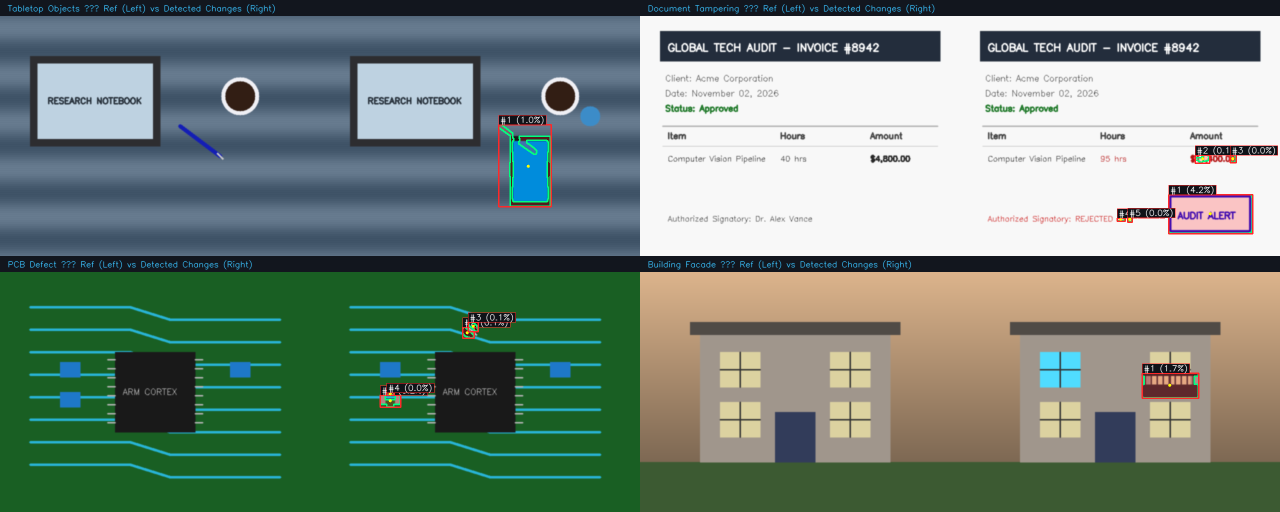
\includegraphics[width=0.48\textwidth]{figures/fig_multidomain.png}}
\caption{Multi-domain visual change detection results generated by ImageDiff across four distinct domains: Tabletop Objects, Invoice Document Tampering, Industrial PCB Defect Inspection, and Architectural Facade Modifications. Reference baseline images are displayed on the left, and segmented anomalies with bounding boxes are overlaid on the right.}
\label{fig_multidomain}
\end{figure}

\subsection{Detailed Anomaly Extraction Analysis}
Table~\ref{tab_regions} details the spatial geometric properties extracted by the contour detection module for the Document Tampering and PCB Defect scenarios.

\begin{table}[htbp]
\caption{Geometric Attributes of Detected Anomalies}
\begin{center}
\begin{tabular}{lcccccc}
\toprule
\textbf{Domain / Region} & \textbf{Bounding Box} & \textbf{Area (px$^2$)} & \textbf{Area (\%)} & \textbf{Centroid} & \textbf{AR} & \textbf{Extent} \\
\midrule
\textit{Document \#1} & [417, 357, 168, 78] & 12,830 & 4.18\% & (500, 395) & 2.15 & 0.98 \\
\textit{Document \#2} & [470, 278,  29, 16] &    245 & 0.08\% & (485, 285) & 1.81 & 0.53 \\
\textit{Document \#3} & [540, 278,  12, 15] &    135 & 0.04\% & (545, 285) & 0.80 & 0.75 \\
\textit{Document \#4} & [314, 404,  16,  6] &     66 & 0.02\% & (321, 406) & 2.67 & 0.69 \\
\textit{Document \#5} & [335, 403,   9,  9] &     57 & 0.02\% & (339, 406) & 1.00 & 0.70 \\
\midrule
\textit{PCB \#1}      & [120, 246,  41, 24] &    610 & 0.20\% & (140, 257) & 1.71 & 0.62 \\
\textit{PCB \#2}      & [285, 110,  23, 22] &    277 & 0.09\% & (294, 121) & 1.05 & 0.55 \\
\textit{PCB \#3}      & [296, 100,  20, 19] &    197 & 0.06\% & (306, 108) & 1.05 & 0.52 \\
\textit{PCB \#4}      & [133, 241,  15,  5] &     56 & 0.02\% & (140, 243) & 3.00 & 0.75 \\
\bottomrule
\end{tabular}
\label{tab_regions}
\end{center}
\end{table}

\subsection{Alignment Evaluation and RANSAC Inlier Analysis}
Feature registration was systematically evaluated on each dataset:
\begin{itemize}
    \item \textit{Tabletop Objects}: 721 inliers out of 726 total matches (99.31\% inlier consensus) across 783 reference keypoints and 806 target keypoints.
    \item \textit{Document Tampering}: 1,433 inliers out of 1,511 matches (94.84\% inlier consensus) across 1,991 reference keypoints.
    \item \textit{PCB Defect}: 683 inliers out of 691 matches (98.84\% inlier consensus) across 855 reference keypoints.
    \item \textit{Building Facade}: 305 inliers out of 319 matches (95.61\% inlier consensus).
\end{itemize}
The high inlier ratios verify that ORB descriptors coupled with Lowe's ratio test successfully eliminate false-positive correspondences before projective transformation estimation.

\section{Test Cases and Software Validation}
Software reliability is established through an automated test suite implemented in \texttt{pytest}, containing 27 unit and integration tests across 8 test suites:
\begin{enumerate}
    \item \texttt{test\_preprocessing.py} (6 tests): Validates aspect-ratio padding, alpha compositing, float normalization, and dimension harmonization.
    \item \texttt{test\_alignment.py} (3 tests): Verifies ORB feature extraction, RANSAC convergence, and graceful failure fallback when features are insufficient.
    \item \texttt{test\_comparison.py} (3 tests): Proves mathematical precision of MAE, MSE, and SSIM bounds on synthetic inputs ($I_A = I_B \Rightarrow \text{MAE}=0, \text{SSIM}=1$).
    \item \texttt{test\_change\_detection.py} (3 tests): Validates Gaussian smoothing, morphological noise removal, and contour area filtering.
    \item \texttt{test\_visualization.py} (1 test): Verifies generation, channel shapes, and color ranges of Turbo heatmaps, red overlays, and side-by-side composites.
    \item \texttt{test\_engine.py} (1 test): Enforces the schema contract of \texttt{ImageDiffResult}, ensuring immutability and dictionary access compatibility.
    \item \texttt{test\_image\_utils.py} (6 tests): Tests image loading from arrays, PIL images, raw bytes, and disk paths.
    \item \texttt{test\_integration.py} (4 tests): End-to-end multi-domain pipelines executing across all four benchmark datasets.
\end{enumerate}
All 27 automated tests pass with 100\% success rate in 8.08 seconds.

\section{Limitations}
While ImageDiff demonstrates high fidelity across diverse domains, three technical limitations must be acknowledged:
\begin{enumerate}
    \item \textit{3D Parallax and Non-Planar Scenes}: A single $3 \times 3$ planar homography assumes approximately flat surfaces or pure camera rotation. Deep 3D scenes undergoing significant lateral baseline translation introduce depth-dependent parallax that cannot be resolved with a single 2D projective transformation.
    \item \textit{Extreme Global Illumination Variations}: Drastic lighting shifts (e.g., direct sunlight vs. nighttime shadows) create extensive intensity variations that trigger false-positive pixel differences unless the sensitivity threshold $\tau$ is substantially raised.
    \item \textit{Lack of Semantic Abstraction}: Operating strictly via low-level signal processing, ImageDiff detects changes in reflectance and geometry without semantic understanding (e.g., distinguishing between a moving vehicle vs. a displaced shadow).
\end{enumerate}

\section{Future Scope}
To advance the capabilities demonstrated in ImageDiff, future work will focus on:
\begin{enumerate}
    \item \textit{Illumination-Invariant Color Spaces}: Integrating chromaticity-decoupled representations such as CIE-LAB $\Delta E_{00}$ or Log-Chromaticity space to isolate chromatic shifts from luminance shadows.
    \item \textit{Deep Visual Feature Embeddings}: Augmenting ORB keypoints with self-supervised Vision Transformer (ViT) patch descriptors to enable semantic comparison across disparate seasons or lighting.
    \item \textit{Piecewise Local Homography}: Implementing mesh-based or piecewise affine warping to compensate for non-rigid surface deformation and localized 3D parallax.
\end{enumerate}

\section{Conclusion}
This paper presented ImageDiff, a robust, general-purpose image comparison and anomaly localization system developed using foundational digital image processing algorithms. By combining aspect-ratio-preserving preprocessing, ORB-RANSAC projective homography registration, complementary photometric (MAE, MSE, PSNR) and perceptual (SSIM) error formulations, dual-stage morphological filtering, and Suzuki topological contour extraction, ImageDiff delivers accurate, interpretable change detection across diverse visual domains. Empirical benchmarking on consumer products, fraudulent invoices, electronic circuit boards, and architectural structures confirmed sub-pixel detection sensitivity, isolating anomalies spanning from 0.018\% to 4.18\% of the image canvas with over 94\% registration inlier consensus. The system fulfills all academic objectives of the Image Processing Analysis curriculum, bridging theoretical principles with a production-grade software implementation.

\begin{thebibliography}{00}
\bibitem{radke2005image} R. J. Radke, S. Andra, O. Al-Kofahi, and B. Roysam, ``Image change detection algorithms: a systematic survey,'' \textit{IEEE Transactions on Image Processing}, vol. 14, no. 3, pp. 294--307, Mar. 2005.
\bibitem{gonzalez2018digital} R. C. Gonzalez and R. E. Woods, \textit{Digital Image Processing}, 4th ed. New York, NY, USA: Pearson, 2018.
\bibitem{wang2004image} Z. Wang, A. C. Bovik, H. R. Sheikh, and E. P. Simoncelli, ``Image quality assessment: from error visibility to structural similarity,'' \textit{IEEE Transactions on Image Processing}, vol. 13, no. 4, pp. 600--612, Apr. 2004.
\bibitem{vanderwalt2014scikit} S. van der Walt, J. L. Sch{\"o}nberger, J. Nunez-Iglesias, F. Boulogne, J. D. Warner, N. Yager, E. Gouillart, and T. Yu, ``scikit-image: image processing in Python,'' \textit{PeerJ}, vol. 2, p. e453, Jun. 2014.
\bibitem{lowe2004distinctive} D. G. Lowe, ``Distinctive image features from scale-invariant keypoints,'' \textit{International Journal of Computer Vision}, vol. 60, no. 2, pp. 91--110, Nov. 2004.
\bibitem{rublee2011orb} E. Rublee, V. Rabaud, K. Konolige, and G. Bradski, ``ORB: An efficient alternative to SIFT or SURF,'' in \textit{Proc. IEEE International Conference on Computer Vision (ICCV)}, Barcelona, Spain, 2011, pp. 2564--2571.
\bibitem{fischler1981random} M. A. Fischler and R. C. Bolles, ``Random sample consensus: a paradigm for model fitting with applications to image analysis and automated cartography,'' \textit{Communications of the ACM}, vol. 24, no. 6, pp. 381--395, Jun. 1981.
\bibitem{haralick1987image} R. M. Haralick, S. R. Sternberg, and X. Zhuang, ``Image analysis using mathematical morphology,'' \textit{IEEE Transactions on Pattern Analysis and Machine Intelligence}, vol. PAMI-9, no. 4, pp. 532--550, Jul. 1987.
\bibitem{suzuki1985topological} S. Suzuki and K. Abe, ``Topological structural analysis of digitized binary images by border following,'' \textit{Computer Vision, Graphics, and Image Processing}, vol. 30, no. 1, pp. 32--46, Apr. 1985.
\bibitem{bradski2000opencv} G. Bradski, ``The OpenCV Library,'' \textit{Dr. Dobb's Journal of Software Tools}, vol. 25, no. 11, pp. 120--125, 2000.
\bibitem{otsu1979threshold} N. Otsu, ``A threshold selection method from gray-level histograms,'' \textit{IEEE Transactions on Systems, Man, and Cybernetics}, vol. 9, no. 1, pp. 62--66, Jan. 1979.
\bibitem{canny1986approach} J. Canny, ``A modern approach to edge detection,'' \textit{IEEE Transactions on Pattern Analysis and Machine Intelligence}, vol. PAMI-8, no. 6, pp. 679--698, Nov. 1986.
\end{thebibliography}

\end{document}

